% Begin of the presentation
\documentclass{beamer}
\usetheme{LEA}
\usepackage{hyperref}
\usepackage{pgf}
\usepackage[utf8]{inputenc}
\usepackage{amsmath}
\usepackage{amsfonts}
\usepackage{amssymb}
\usepackage{amsthm}
\usepackage{graphicx}
\graphicspath{{media/}}
%\usepackage[shortend]{algorithm2e}
\usepackage{multicol}
\usepackage{tikz}
\usetikzlibrary{shapes,positioning}
\usepackage{soul}

% configuration to insert java code "https://stackoverflow.com/questions/3175105/inserting-code-in-this-latex-document-with-indentation"
\usepackage{listings}
\usepackage{color}

\definecolor{dkgreen}{rgb}{0,0.6,0}
\definecolor{gray}{rgb}{0.5,0.5,0.5}
\definecolor{mauve}{rgb}{0.58,0,0.82}
\lstset{frame=tb,
  language=Java,
  aboveskip=3mm,
  belowskip=3mm,
  showstringspaces=false,
  columns=flexible,
  basicstyle={\small\ttfamily},
  numbers=none,
  numberstyle=\tiny\color{gray},
  keywordstyle=\color{blue},
  commentstyle=\color{dkgreen},
  stringstyle=\color{mauve},
  breaklines=true,
  breakatwhitespace=true,
  tabsize=3
  }
\usepackage [backend=biber,style=authortitle]{biblatex}
\bibliography{presentation.bib}

%                          Information for the Title Page
%
\title[Deductive Verification]{
	\Large Deductive Verification : An Axiomatic Basis for Computer Programming by C.A.R Hoare\\
	[5mm] \normalsize Sarntal Ferienakademie -- Course 1 \\
	Modern Approaches to Optimization and Verification in Computer Science
}
\author{Rayen Manai}


% uncomment appropriate affiliation
\institute[]{
    TU München\\
%    FAU Erlangen-Nürnberg\\
%    Universität Stuttgart\\
}
\date{18.09.2022 -- 30.09.2022}
\titlegraphic{%
	\vspace{5mm}%
	
\includegraphics[height=7mm]{FAU_TechFak_Q_RGB_black}%
	\hspace{10mm}%
	
\includegraphics[height=7mm]{tum_logo}%
	\hspace{10mm}%
	
\includegraphics[height=7mm]{stuttgart_logo}%
}


%                                Beginning of the document 
%
\begin{document}
\begin{frame}
	\titlepage
\end{frame}

\begin{frame}
	\frametitle{Outline}
	\tableofcontents
\end{frame}

%---------------------------------------------------------------------- SLIDE -
\section{Introduction}
\begin{frame}
 \begin{center}
                Why do we need to verify our programs?
        \end{center}

\end{frame}
	\begin{frame}
\center
  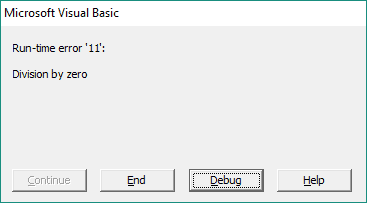
\includegraphics[height=45mm]{error}
	\end {frame}
	\begin{frame}
 \center 

\includegraphics[height=45mm]{social_network}
\end{frame}

%---------------------------------------------------------------------- SLIDE -
\begin{frame}
        \frametitle{Software is hard - Don Knuth}
Why?
\begin{itemize}

  \item {wrong interpretation of specifications}
  \item {coding in a hurry}
  \item {incompatible changes}
  \item {software = complex artifact}

\end{itemize}
\end{frame}

%---------------------------------------------------------------------- SLIDE -
\begin{frame} [fragile]
	\frametitle{Binary Search}
	\center
\begin{lstlisting}
public static int binarySearch(int[] a, int key) {
	int low = 0;
	int high = a.length - 1;
	 while (low <= high) {
		 int mid = (low + high) / 2;
		 int midVal = a[mid];
		 if (midVal < key)
		 low = mid + 1
		 else if (midVal > key)
		 high = mid - 1;
		 else
		 return mid; // key found
		 }
		 return -(low + 1);  // key not found.
		 }

\end{lstlisting}
\end{frame}

%---------------------------------------------------------------------- SLIDE -
\begin{frame} [fragile]
        \frametitle{Binary Search}

        \center
\begin{lstlisting}
public static int binarySearch(int[] a, int key) {
        int low = 0;
        int high = a.length - 1;
         while (low <= high) {
\end{lstlisting}
\vspace{-\baselineskip}
\begin{lstlisting}[backgroundcolor=\color{pink}]
int mid = (low + high) / 2; // if low + high > MAX_INTEGER: Overflow
int midVal = a[mid]; // Array Access not safe
\end{lstlisting}
\vspace{-\baselineskip}
\begin{lstlisting}
                 if (midVal < key)
                 low = mid + 1
                 else if (midVal > key)
                 high = mid - 1;
                 else
                 return mid; // key found
                 }
                 return -(low + 1);  // key not found.
                 }

\end{lstlisting}
\end{frame}

%---------------------------------------------------------------------- SLIDE -
\begin{frame} [fragile]
        \frametitle{Binary Search}

        \center
\begin{lstlisting}
public static int binarySearch(int[] a, int key) {
        int low = 0;
        int high = a.length - 1;
         while (low <= high) {
\end{lstlisting}
\vspace{-\baselineskip}
\begin{lstlisting}[backgroundcolor=\color{green}]
int mid = low + ((high - low) / 2); 
int midVal = a[mid]; 
\end{lstlisting}
\vspace{-\baselineskip}
\begin{lstlisting}
                 if (midVal < key)
                 low = mid + 1
                 else if (midVal > key)
                 high = mid - 1;
                 else
                 return mid; // key found
                 }
                 return -(low + 1);  // key not found.
                 }

\end{lstlisting}
\end{frame}
%---------------------------------------------------------------------- SLIDE -

\begin{frame}
 \begin{center}
                But how do we measure software correctness?
        \end{center}

\end{frame}

%---------------------------------------------------------------------- SLIDE -
\section{Testing vs Verification}
\begin{frame}
        \frametitle{Testing Vs. Verification}
	\begin{minipage}[t]{0.48\linewidth}
        Testing
		\begin{itemize}
            \item Run the system at chosen inputs and observe its behavior
            \item Randomly chosen – Intelligently chosen (by hand: expensive!)
      	\item  Automatically chosen (need formalized spec.)
            \item What about other inputs? (test coverage)
        \end{itemize}
    \end{minipage}
    \hfill
	\pause
    \begin{minipage}[t]{0.48\linewidth}
        Verification
        \begin{itemize}
            \item Logical reasoning
            \item mathematical proof techniques
            \item establish properties about programs
	    \item all possible behaviors for all possible inputs
        \end{itemize}
    \end{minipage}
\end{frame}



%---------------------------------------------------------------------- SLIDE -
\section{Verification}
\begin{frame}
        \frametitle{Verification}
\begin{itemize}

  \item {Deductive software verification = program proving}
  \item {Correctness of a program as a set of mathematical statements, called verification
conditions}
  \item {Process of turning the correctness of a program into a mathematical statement and then
proving it}
  \item {The idea is not new. It is actually as old as programming}

\end{itemize}

\end{frame}


%---------------------------------------------------------------------- SLIDE -
\section{Ingredients: Axioms and Theorems}
\begin{frame}
        \frametitle{Ingredients: Axioms and Theorems}
	“In this paper an attempt is made to explore the logical foundations of computer programming
	by use of techniques which were first applied in the study of \colorbox{yellow!30}{geometry} and have later been
	extended to other branches of mathematics. This involves the elucidation of sets of \colorbox{blue!30}{axioms}
	and\colorbox{blue!30}{rules of inference} which can be used in proofs of the properties of computer programs.” - Tony Hoare
\end{frame}

%---------------------------------------------------------------------- SLIDE -
\begin{frame}
\begin{minipage}[t]{0.48\linewidth}
	Axioms
                \begin{itemize}
            \item axiom = postulate = assumption
            \item a statement that is taken to be true
        \item  serve as a premise or starting point for further reasoning and arguments
            \item The set of facts we have to work with
        \end{itemize}
    \end{minipage}
    \hfill
        \pause
    \begin{minipage}[t]{0.48\linewidth}
	    Theorems
        \begin{itemize}
            \item a statement that has been proved
            \item or can be proved by a logical argument
            \item uses the inference rules of a deductive system
            \item logical consequence of the axioms and previously proved theorems
        \end{itemize}
    \end{minipage}
\end{frame}
%---------------------------------------------------------------------- SLIDE -
\section{Notation: Hoare triple}
\begin{frame}
        \frametitle{Notation: Hoare triple}
$$  P \; \{Q\} \; R $$
\begin{itemize}
            \item P : Precondition
            \item R : Postcondition
\item "If the assertion P is true before initiation of a program Q, then the
assertion R will be true on its completion." 
\item If there are no preconditions imposed, we write: $true \;
\{Q\} \; R$
		\end {itemize}
\end{frame}

%---------------------------------------------------------------------- SLIDE -
\begin{frame}
        \frametitle{Examples}
	\begin{itemize}
		\item $$ x > y \; \{ z = x-y;\} \; z > 0 $$
                \item $$ true \;  \{if(x<0) \, x = -x ;\} \; x >= 0 $$
		\item $$ x > 5 \; \{ while(x \neq 0) \; x = x - 1;\} \; x = 0 $$
                \item $$ true \;  \{while(true)\} \; false $$
		\item   $$ false \;  \{x = 4\} \; x = 7 $$
			\end{itemize}
\end{frame}


%---------------------------------------------------------------------- SLIDE -
\section{Axioms and rules}
\begin{frame}
        \frametitle{Axioms and rules} 
	$$A1: \; \; x \; + \; y \; = y \; + \; x $$
	$$A2: \; \; x \; \times \; y \; = y \; \times \; x $$
        $$A3: \; \; (x \; + \; y) \; + \; z  \; = x \; + \;(y \; + \; z)  $$
        $$A4: \; \; (x \; \times \; y) \; \times \; z  \; = x \; \times \;(y \; \times \; z)  $$
	$$A5: \; \; x \; \times \; (y \; + \; z)  \; = x \; \times \;y \; + \; x \; \times \; z  $$
	$$A6: \; y \; \leq \; x \; \implies \; (x \; - \; y) \; + \; y \; = \; x $$
	$$A7: \; x \; + \; 0 \; = \; x $$
	 $$A8: \; x \; \times \; 0 \; = \; 0 $$
	 $$A9: \; x \; \times \; 1 \; = \; x $$

\end{frame}


%---------------------------------------------------------------------- SLIDE -
\subsection{Axiom of assignment}
\begin{frame}
        \frametitle{Axiom of assignment}
	$$  P_{0} \; \{x := f \} \; P $$
\begin{itemize}
            \item  $x$ : variable identifier
            \item $f$ : an expression
\item $P_{0}$ is obtained from $P$ by substituting $f$ for all occurences of $x$
                \end {itemize}
\pause
Examples: 
		$$ x = y \; \{ x =\colorbox{blue!30}{ x + 3};\} \;\colorbox{blue!30} {x} = y + 3 $$
\end{frame}


%---------------------------------------------------------------------- SLIDE -
\subsection{Rule of consequence}
\begin{frame}
        \frametitle{Rule of consequence}
	\begin{itemize}
		\item $$ \textrm{if} \; (P \; \{Q\} \; R \; \; \land \; R \implies S) \; \textrm{then} \; P \; \{Q\} \; S $$
		\item $$ \textrm{if} \; (P \; \{Q\} \; R \; \; \land \; S \implies P) \; \textrm{then} \; S \; \{Q\} \; R $$
	\end{itemize}
\pause
        Examples:
	$$\colorbox{yellow!30}{ x $>$ 1} \; \{ x = x + 1;\} \; x > 2 $$
	$$\colorbox{yellow!30} {x $>$ 3} \implies x > 1 $$
	$\rightarrow $ $$\colorbox{yellow!30}{ x $>$ 3} \; \{ x = x + 1;\} \; x > 2 $$
\end{frame}

%---------------------------------------------------------------------- SLIDE -
\subsection{Rule of composition}
\begin{frame}
        \frametitle{Rule of composition}
	 \begin{itemize}
		 \item $$ \textrm{if} \; (P \; \{Q_{1}\} \; R_{1} \; \; \land \; R_{1} \; \{Q_{2}\} \; R) \; \textrm{then} \; P \; \{Q_{1};Q_{2}\} \; R $$
	 \end{itemize}
\pause
Examples: 
	$$ x > 1 \; \{ x = x + 1;\} \;\colorbox{blue!30} {x $>$ 2} $$
	$$\colorbox{blue!30}{ x $>$ 2} \; \{ x = x + 1;\} \; x > 3 $$
  $\rightarrow $ $$ x > 1 \; \{ x = x + 1; x = x + 1; \} \; x > 3 $$
	\pause
	\hrule
	$$ x > 1 \; \{ x = x + 1;\} \;\colorbox{blue!30} {x $>$ 2} $$
	$$\colorbox{blue!30}{ x $>$ 0} \; \{ x = -x;\} \; x < 0 $$
  $\rightarrow $ $$ x > 1 \; \{ x = x + 1; x = -x; \} \; x < 0 $$


\end{frame}
%---------------------------------------------------------------------- SLIDE -
\subsection{Rule of iteration}
\begin{frame}
        \frametitle{Rule of iteration}
	\begin{itemize}
		\item $$\textrm{if} \; (P \; \, \land \; \, B \; \{S\} \; P) \;\textrm{then} \; P \; \{while \; B \; do \; S \; \} \; \neg B \, \land \; P $$
		\item B : the controlling condition
		\item P : Loop Invariant: an assertion which is always true on completion of S, provided that it is also true on initiation. Then obviously P will still be true after any number of iterations of the statement S.
	\end{itemize}
	\pause
	Examples :
	$$ x > 0 \; \{ while(x<10) \; do \; x = x + 1;\} \; x \geq 10 \; \land \; x > 0 $$
\end{frame}

%---------------------------------------------------------------------- SLIDE -
\section{Proof example}
	\begin{frame}[fragile] 
 \frametitle{Proof example}
	"The axioms quoted above are sufficient to construct the proof of properties of simple
programs, for example, a routine intended to find the quotient q and remainder r obtained on
dividing x by y. All variables are assumed to range over a set of nonnegative integers
conforming to the axioms listed in Table I"
The proposed program is: 
\center
\begin{lstlisting}
    r = x;
    q = 0;
    while (y <= r) {
	    r = r - y;
	    q = q + 1;
	    }
\end{lstlisting}

\end{frame}

%---------------------------------------------------------------------- SLIDE -
\begin{frame}[label = controlflow, squeeze ]
	\frametitle{control flow}
	\center
	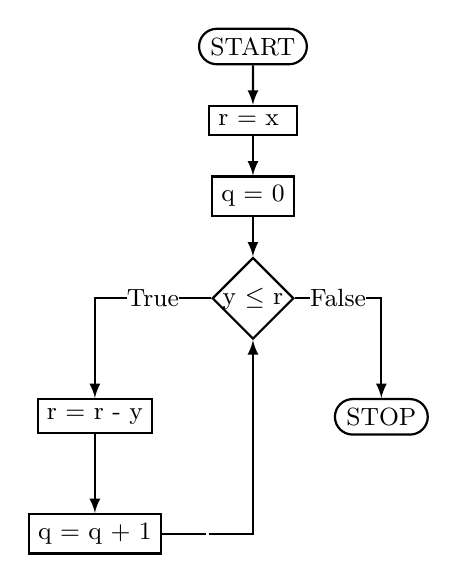
\begin{tikzpicture}[font=\small,thick]
% Start block
\node[draw,
    rounded rectangle,
    ] (block1) {START};

% Assignments block
\node[draw,
    align = center,
    below= 5mm of block1
] (block2) { r = x };

\node[draw,
    align=center,
    below= 5mm of block2
] (block3) { q = 0};

% Conditions test
\node[draw,
    diamond,
    below= 5mm of block3,
		inner sep=0] (block4) {y $ \leq$ r};

\node[draw,
    below left=of block4
		] (block5) {r = r - y};

\node[draw,
    below=of block5] (block6) { q = q + 1};

%Stop block
\node[draw,
    rounded rectangle,
    below right = of block4
		] (block7) {STOP};

% Arrows
\draw[-latex] (block1) edge (block2)
    (block2) edge (block3)
    (block3) edge (block4)
		(block5) edge (block6);
\draw[-latex] (block4) -| (block5)
    node[pos=0.25,fill=white,inner sep=0]{True};
\draw[-latex] (block6) -| (block4)
    node[pos=0.25,fill=white,inner sep=0]{};
\draw[-latex] (block4) -| (block7)
    node[pos=0.25,fill=white,inner sep=0]{False};

\end{tikzpicture}
\end{frame}

%---------------------------------------------------------------------- SLIDE -
\begin{frame}
\frametitle{Approach}
\begin{itemize}
\item When the program terminates the numerator $x$ can be recovered by: $$ x \; = r \; + \; y \; \times \; q $$
\item The remainder is less than the divisor: $$ r < y $$ 
\item Loop Invariant: $$ x \; = r \; + \; y \; \times \; q $$
\item Our goal: $$  true \; \{Q\} \; \neg \; y\leq r\; \; \land \; x\; = \; r\; + \; y \times q $$
\end{itemize}

\end{frame}
%------------------------------------------------------------

\begin{frame}[label = controlflow, squeeze ]
	\center
	\colorbox{green!30}{A = True} 
	, \colorbox{blue!30}{B = $\neg \; y\leq r\; \; \land \; x\; = \; r\; + \; y \times q $}
        \center
        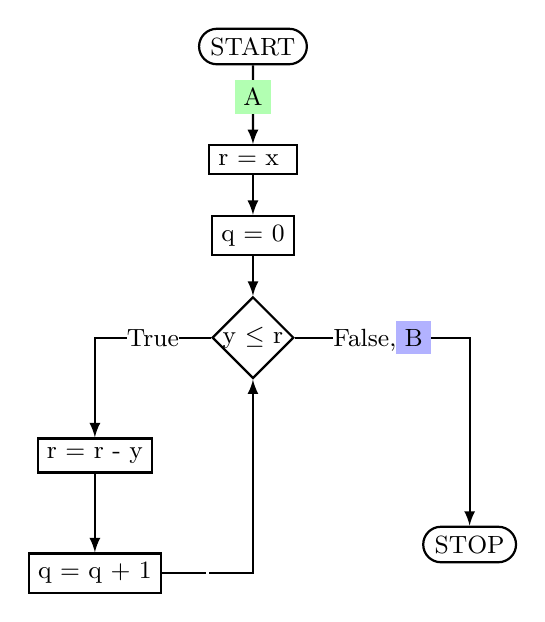
\begin{tikzpicture}[font=\small,thick]
% Start block
\node[draw,
    rounded rectangle,
    ] (block1) {START};

% Assignments block
\node[draw,
    align = center,
    below= 10mm of block1
] (block2) { r = x };

\node[draw,
    align=center,
    below= 5mm of block2
] (block3) { q = 0};

% Conditions test
\node[draw,
    diamond,
    below= 5mm of block3,
                inner sep=0] (block4) {y $ \leq$ r};

\node[draw,
    below left=of block4
                ] (block5) {r = r - y};

\node[draw,
    below=of block5] (block6) { q = q + 1};
%Stop block
\node[draw,
    rounded rectangle,
    below right = 3 cm  of block4
                ] (block7) {STOP};

% Arrows
\draw[-latex]
    (block2) edge (block3)
    (block3) edge (block4)
                (block5) edge (block6);
	
\draw[-latex] (block1) -- (block2)
		node[pos=0.4,fill=white,inner sep=0]{\colorbox{green!30}{A}};
\draw[-latex] (block4) -| (block5)
    node[pos=0.25,fill=white,inner sep=0]{True};
\draw[-latex] (block6) -| (block4)
    node[pos=0.25,fill=white,inner sep=0]{};
\draw[-latex] (block4) -| (block7)
		node[pos=0.25,fill=white,inner sep=0]{False,\colorbox{blue!30} {B}};

\end{tikzpicture}
\end{frame}



%-----------------------------------------------------

\begin{frame}
	\center
	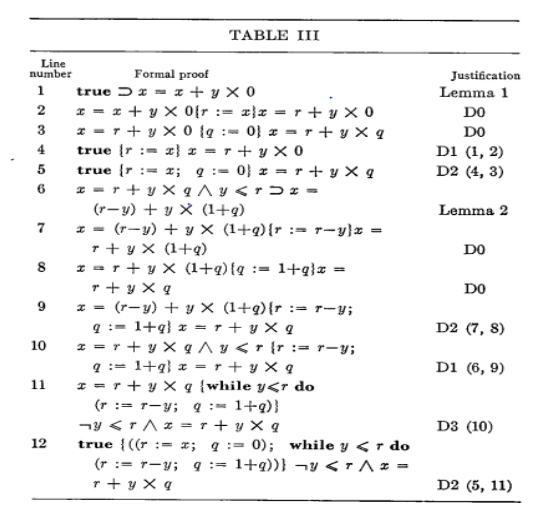
\includegraphics[width = 8.5cm] {proof1.png}
\end{frame}
\begin{frame}
        \center
        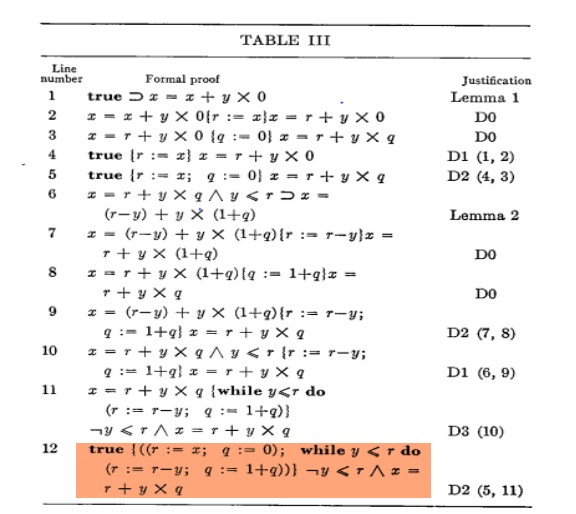
\includegraphics[width = 8.5cm] {proof2.png}
\end{frame}
\begin{frame}
        \center
        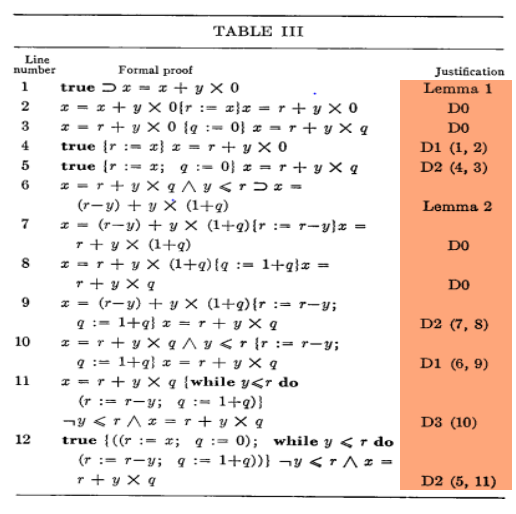
\includegraphics[width = 8.5cm] {proof3.png}
\end{frame}
\begin{frame}
        \center
        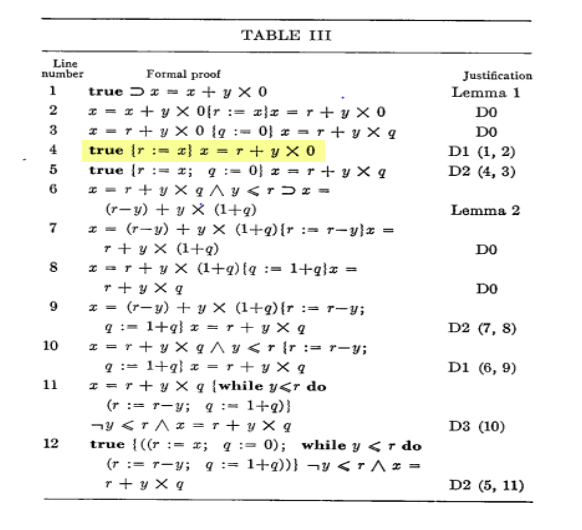
\includegraphics[width = 8.5cm] {proof4.png}
\end{frame}

%---------------------------------------------------------------------- SLIDE -
\section{Discussion}
\subsection{Advantages}
\begin{frame}
        \frametitle{Advantages}
        \begin{itemize}
                \item Program documentation
                \item Program modification
                \item Program portability
                \item Program reliability
         \end{itemize}
        \pause
	\center
        But...
        \end{frame}

%---------------------------------------------------------------------- SLIDE -
\subsection{Challenges}
\begin{frame}
        \frametitle{Challenges}
	\begin{itemize}
		\item Real World vs Formal World: missing requirement eg, stack overflow
		\item Difficulty of writing formal proofs 
		\item Difficulty of finding Loop Invariants 
		\item Dependency on implementation features
		\item Termination?
		\item Side effects?
         \end{itemize} 
	\pause
	“The practice of supplying proofs for nontrivial programs will not become widespread until
considerably more powerful proof techniques become available, and even then will not be
easy. But the practical advantages of program proving will eventually outweigh the difficulties,
in view of the increasing costs of programming error.” -Tony Hoare
	\end{frame}

%---------------------------------------------------------------------- SLIDE -
\section{Verification Tools based on Hoare Logic}
\begin{frame}
        \frametitle{Verification Tools based on Hoare Logic}
	\center
	
\includegraphics[width=25mm] {isabelle}
\hspace{15mm}
	
\includegraphics[width=25mm] {Z3.jpeg}
	\newline
	\vspace {20mm}
        
\includegraphics [width=25mm] {coq}
	\hspace{15mm}
	
\includegraphics [width=25mm] {TLA+}


\end{frame}

%---------------------------------------------------------------------- SLIDE -
\begin{frame}
	\frametitle{TLA+ used by AWS}
	\begin{itemize}
\item “At AWS, formal methods have been a big success. They have helped us prevent subtle,
serious bugs from reaching production, bugs that we would not have found via any other
technique. They have helped us to make aggressive optimizations to complex algorithms
without sacrificing quality.”

\item “... We believe that use of TLA+ will accelerate both time-to-market and quality of these
	projects” \footfullcite{TLA+}
\end{itemize}
\end{frame}	

\begin{frame}
        \frametitle{The seL4 Microkernel}
        \center
	
\includegraphics[width = 60mm] {sel4.png}
	\footfullcite{sel4}
\end{frame}
%---------------------------------------------------------------------- SLIDE -

\section{Conclusion}
\begin{frame}
	\frametitle{Conclusion}
	\begin{itemize}
		\item Always think about correctness
		\item Importance of verification (safety-critical applications)
		\item Hoare's contributions to software verification 
		\item Hoare's triple
		\item A way of characterising programs and properties
		\item Formal methods in praxis and challenges
		\item Automated tools to check program properties
	\end{itemize}
\end{frame}

%---------------------------------------------------------------------- SLIDE -
\begin{frame}
	\begin{center}
		Thank you!
	\end{center}
\end{frame}
\printbibliography
\end{document}
